\documentclass[14pt]{article}
\usepackage{ucs}
\usepackage[utf8x]{inputenc}
\usepackage[russian]{babel}  
\usepackage{amsmath}
\usepackage{amssymb}
\usepackage{mathtools}
\usepackage{hyperref}
\usepackage{graphicx}
\usepackage{caption}
\usepackage{xcolor}
\usepackage{hyperref}

% Цвета для гиперссылок
\definecolor{linkcolor}{HTML}{00008B} % цвет ссылок
\definecolor{urlcolor}{HTML}{00008B} % цвет гиперссылок
 
\hypersetup{pdfstartview=FitH,  linkcolor=linkcolor,urlcolor=urlcolor, colorlinks=true}

\graphicspath{{pictures/}}

\DeclareGraphicsExtensions{.pdf,.png,.jpg}

\newtheorem{Def}{Определение}

\newtheorem{Fact}{Факт}

\newtheorem{Th}{Теорема}

\newtheorem{Lem}{Лемма}

\newenvironment{PROOF}
{\par\noindent{\bf Доказательство:}\newline$\triangleright$}
{\hfill$\scriptstyle\blacktriangleleft$}

\linespread{1.3}
\hoffset=0mm
\voffset=0mm
\textwidth=160mm 
\oddsidemargin=0mm   
\textheight=240mm       
\topmargin=-15.4mm      
\headheight=5mm     
\headsep=5mm          
\footskip=8mm        

\title{
\textbf{Метрическая задача коммивояжёра - 1} 
}

\date{\today}
\author{Ткаченко Дмитрий}

\begin{document}

    \maketitle
    
    \begin{figure}[h]
		\center{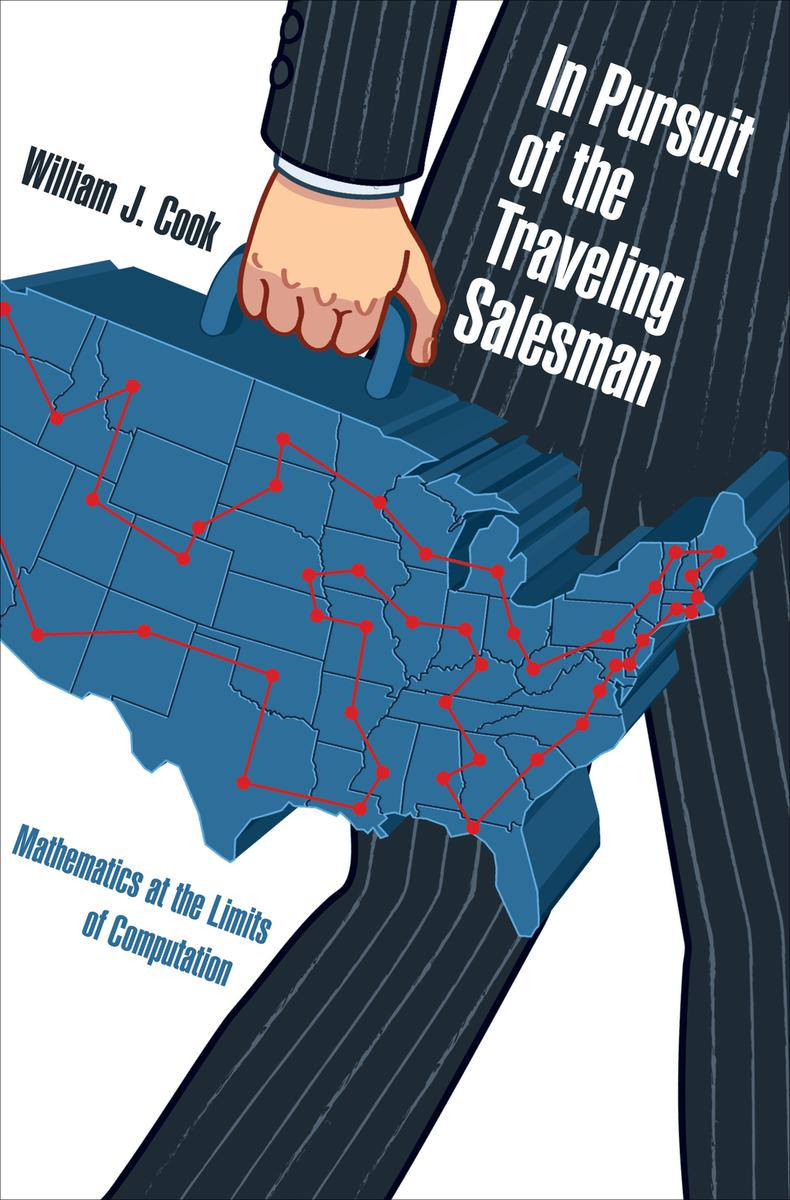
\includegraphics[scale=0.4]{in-pursuit-of-the-traveling-salesman.jpg}}
		\caption*{\hyperref[book1]{In Pursuit of the Traveling Salesman}}
	\end{figure}
	
	\tableofcontents
	
	%----------------------------------------------------------
	
	\section{Введение}
		Проблема коммивояжёра - одна из самых известных задач комбинаторной оптимизации, с которой ежедневно сталкиваются курьеры, почтальоны, путешественники. Их цель - найти наиболее выгодный маршрут, проходящий через заранее известные места, расстояния между которыми тоже известны. В данной работе рассмотрен метрический случай данной задачи и алгоритмы нахождения её приближенного решения.
		
	%----------------------------------------------------------
		
	\section{Поставленные задачи и вопросы}
	
		\begin{enumerate}
			\item[$($а$)$] Несуществование полиномиального алгоритма для стандартной задачи коммивояжера, дающего константное приближение, в предположении \textbf{P} $\ne$ \textbf{NP}.
			\item[$($б$)$] Построение алгоритма, дающего 2-приближение для метрической задачи коммивояжёра на основе остовного дерева.
			\item[$($в$)$] Построение алгоритма, дающего 1.5-приближение для метрической задачи коммивояжёра на основе остовного дерева и паросочетания. 
			\item[$($г$)$] Реализация алгоритма, дающего 1.5-приближение для метрической задачи коммивояжёра.
		\end{enumerate}
		
	%----------------------------------------------------------
		
	\section{Теория и необходимые определения}
		
		Для начала сформулируем \textbf{общую задачу коммивояжёра}: в данном взвешенном графе $G = (V, E)$ с весами на рёбрах $w: V \times V \rightarrow \mathbb{R}_+$ найти гамильтонов цикл минимального веса.
		
		\begin{center}
			\textbf{\large Определения из теории графов:}
		\end{center}
		
		\begin{Def}
			\textbf{Путем} в графе $G = (V, E)$ называется упорядоченный список $(v_1, e_1, v_2, \dots, e_{k-1}, v_k)$ (иногда ребра в записи опускают), где любые две соседствующие в списке вершины $v_i$ и $v_j$ соединены ребром, записанным между ними.
		\end{Def}

		\begin{Def}
			\textbf{Циклом} в графе $G = (V, E)$ называется путь, в котором $v_1 = v_k$.
		\end{Def}
		
		\begin{Def}
			Цикл в графе $G = (V, E)$ называется \textbf{простым}, если все вершины и ребра в нем встречаются не более, чем один раз.
		\end{Def}

		
		\begin{Def}
			Цикл в графе называется \textbf{гамильтоновым}, если он проходит через все вершины графа ровно по одному разу.
		\end{Def}
		
		\begin{Def}
			Граф $G = (V, E)$ с функцией весов $w : V \times V \rightarrow \mathbb{R}_+$ называется \textbf{метрическим}, если $\forall x,y,z \in V $ выполнено (неравенство треугольника) $ w(x, z) \leq w(x, y) + w(y, z)$.
	
		\end{Def}
		
		\begin{Def} 
			Связный граф без простых циклов называется \textbf{деревом}.
		\end{Def}

		\begin{Def}
			Подграф $H$ в графе $G = (V, E)$ называется \textbf{остовным деревом}, если $H$ - дерево и множество вершин $H$ совпадает с множеством вершин $G$.	
		\end{Def}
		
		\begin{center}
			\textbf{\large Определения из сложности вычислений:}
		\end{center}
		
		\begin{Def}
			Классом \textbf{DTIME}$(T(n))$ называется класс языков, которые распознаются за время $O(T(n))$.	
		\end{Def}
		
		\begin{Def}
			Классом \textbf{NTIME}$(T(n))$ называется класс языков, которые распознаются на недетерминированной машине Тьюринга за время $O(T(n))$.	
		\end{Def}

		
		\begin{Def}
			Классом \textbf{P} называется множество языков, которые распознаются за полиномиальное время, или, более формально, $\textbf{P} = \bigcup_{c=1}^\infty \textbf{DTIME}(n^c)$	
		\end{Def}

		\begin{Def}
			Класс \textbf{NP} есть 	$\textbf{NP} = \bigcup_{c=1}^\infty \textbf{NTIME}(n^c)$.
		\end{Def}

		
		\begin{Def}
			Язык $A$ называется \textbf{NP}-\textbf{полным}, если для $\forall B \in \textbf{NP}$  существует полиномиально вычислимая функция $f_B : \{0, 1\}^* \rightarrow \{0, 1\}^*$ такая, что $\forall x \in \{0, 1\}^* : x \in A \Leftrightarrow f_B(x) \in B$.
		\end{Def}
		
		\begin{Def}
			\textbf{Метрической задачей коммивояжера} называется язык пар $L = \{ (G, k)|$ в метрическом графе G с заданными весами ребер существует гамильтонов цикл веса не более k$\}$.	
		\end{Def}
		
		\begin{Fact}
			Язык HAMCYCLE $= \{ G |$ в графе G существует гамильтонов цикл$\}$ является $\textbf{NP}$-полным.	
		\end{Fact}

		
		\begin{center}
			\textbf{\large Определения из теории алгоритмов:}
		\end{center}
	
		\begin{Def}
			Полиномиальный алгоритм дает \textbf{c}-приближение, если результат его работы отличается от верного не более, чем в \textbf{c} раз.	
		\end{Def}

		
	%----------------------------------------------------------	
	
	\section{Несуществование алгоритма, дающего константное приближение для стандартной задачи коммивояжёра}
	
	Этот раздел будет представлен лишь теоремой из заглавия:
	
	\begin{Th}
		(В предположении $\textbf{P} \ne \textbf{NP}$) Для стандартной задачи коммивояжера не существует алгоритма, дающего константное приближение и работающего за полиномиальное время.	
	\end{Th}
	
	\begin{PROOF}
	Предположим, что такой алгоритм существует (назовем его $A$) и дает $c$-приближение. Построим с помощью него полиномиальный алгоритм, который определяет принадлежность графа $G$ к языку HAMCYCLE.
	
	Рассмотрим произвольный граф $G = (V, E)$. Достроим его до полного взвешенного графа $Q$. Ребрам, которые входили в $G$, сопоставим вес 1, а всем остальным дадим вес $|V|c + 1$. Применим $A$ к новому графу $Q$. Результат - гамильтонов цикл $H$ веса $w(H)$.
	
	Пусть $w(H) \leq |V|c$. В таком случае кратчайший гамильтонов цикл имеет вес $w_{opt} \leq w(H)$, а значит в нем нет новых ребер (так как вес каждого из них превосходит $w(H)$), тогда $H$ присутствовал и в графе $G$.
	
	Пусть $w(H) > |V|c$, тогда наименьший гамильтонов цикл имеет вес $w_{opt} \geq \frac{w(H)}{c} > |V|$, значит он содержит хотя бы одно новое ребро, но тогда в исходном графе гамильтонова цикла не было (его вес равен $|V|$).
	
	Таким образом, предъявлен способ решения \textbf{NP}-полной задачи с помощью полиномиального алгоритма, а значит $\mathbf{P} = \mathbf{NP}$, что противоречит предположению $\mathbf{P} \ne \mathbf{NP}$.	
	\end{PROOF}

	%----------------------------------------------------------
	
	\section{Алгоритм, дающий 2-приближение для метрической задачи}
	
	Для метрической (в отличие от стандартной) задачи коммивояжёра существуют алгоритмы, дающие константное приближение. Для начала рассмотрим алгоритм, дающий 2-приближение, а затем обратимся к алгоритму Кристофидеса \hyperref[algoChrist]{$^{[2]}$} и реализуем его.
	
	\begin{Th}\label{Th2}
		Пусть дан произвольный полный взвешенный метрический граф $G = (V,E)$ и цикл $C$, проходящий по всем его вершинам (возможно, не раз). Тогда граф $G$ содержит гамильтонов цикл веса $w_{Ham} \leq w(C)$.	
	\end{Th}
	
	\begin{PROOF}
		Пусть $C = \{v_0,\dots, v_k\}$. Оставим в $C$ вершины лишь в позициях их первого вхождения. Тогда получим какой-то гамильтонов цикл $H$ в графе $G$. Оценим $w(H)$. При выкидывании вершин между $l$-ой и $r$-ой получили замену рёбер $(v_l,v_{l+1}), (v_{l+1}, v_{l+2}), \dots, (v_{r-1}, v_r)$ на ребро $(v_l, v_r)$. По неравенству треугольника имеем: $w(v_l, v_r) \leq w(v_l, v_{l+1}) + w(v_{l+1}, v_r) \leq \dots \leq w(v_l, v_{l+1}) + w(v_{l+1}, v_{l+2}) + \dots + w(v_{r-1}, v_r)$. Отсюда следует, что $w(H) \leq w(C)$. 
	\end{PROOF}
	
	\begin{center}
		\textbf{\large Обратимся теперь к самому алгоритму:}
	\end{center}

	\begin{enumerate}
		\item В данном графе $G=(V,E)$ найдем остовное дерево минимального веса $T$ (это делается за полином с помощью алгоритма Краскала или алгоритма Прима).
		\item Зафиксируем произвольную вершину $T$, обозначим ее $v_0$. Подвесим за нее наше дерево и запустим из нее обход в глубину: рекурсивно обходим поддеревься, после чего возвращаемся в предка. Обход работает до тех пор, пока все вершины не будут посещены и обход не вернется в $v_0$.\center{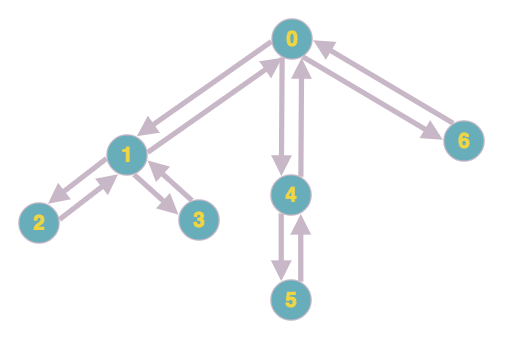
\includegraphics[scale=0.4]{DFS.png}}
	\end{enumerate}
	
	Получим цикл $K$, в котором встречаются все вершины нашего графа, причем $w(K) = 2w(T)$, так как каждое ребро мы посещаем в момент входа в вершину и момент выхода из нее. Таким образом по \hyperref[Th2]{теореме 2} получаем, что в нашем графе есть гамильтонов цикл $H$ такой, что $w(H) \leq w(K) \leq 2w(T)$. Построить сам цикл $H$ мы можем по доказательству \hyperref[Th2]{теоремы 2}.
	
	Какое приближение у нашего алгоритма? Пусть $\hat{H}$ - гамильтонов цикл минимального веса. $w(\hat{H}) \geq w(T)$, так как если убрать любое ребро из $\hat{H}$, то получим какое-то остовное дерево $G$, а $T$ - остовное дерево минимального веса. Тогда $w(\hat{H}) \geq w(T) = \frac{w(H)}{2}$. Таким образом, $w(H) \leq 2w(\hat{H})$, значит наш алгоритм дает 2-приближение метрической задачи коммивояжёра.
	
	%----------------------------------------------------------
	
	\section{Алгоритм, дающий 1.5-приближение для метрической задачи}
	
	Рассмотрим алгоритм Кристофидеса\hyperref[algoChrist]{$^{[2]}$}:
	
	\begin{enumerate}
		\item Находим минимальное остовное дерево $T$.
		\item Выделяем в дереве $T$ подмножество вершин $N(T)$ нечетной степени. В полном графе $G$ среди вершин $N(T)$ ищем совершенное паросочетание $M$ минимального веса. (делается за полиномиальное время с помощью \hyperref[kolm]{blossom-алгоритма})
		\item Построим Эйлеров граф $G_E$ на вершинах $V(G)$ и ребрах $E(T) \cup E(M)$. Он Эйлеров, так как у каждой вершины нечетной степени мы добавили по ребру $\Rightarrow$ степени всех вершин четны $\Rightarrow$ граф эйлеров.
		\item Строим Эйлеров цикл $K$ в графе из предыдущего пункта. (ему естественным образом соответствует цикл $U$, проходящий по всем вершинам)
		\item Строим Гамильтонов цикл $H$ из цикла $U$ как описывает это \hyperref[Th2]{теорема 2}.
	\end{enumerate}
	
	\begin{Th}
		Описанный выше алгоритм Кристофидеса даёт 1.5-приближение для метрической задачи коммивояжёра.	
	\end{Th}
	
	\begin{PROOF}
		Заметим, что справедлива оценка $w(H) \leq w(U) \leq w(T) + w(M)$. Рассмотрим гамильтонов цикл $L$ на вершинах из $M$. Аналогично \hyperref[Th2]{теореме 2} $w(L) \leq w(\hat{H})$ (где $\hat{H}$ - гамильтонов цикл в $G$ минимального веса), причем $L$ - объединение двух непересекающихся паросочетаний  в графе, индуцированном на вершины $M$. Вес каждого из них не менее, чем вес минимального паросочетания $M$, значит $2w(M) \leq w(L) \leq w(\hat{H}) \Rightarrow w(M) \leq \frac{w(\hat{H})}{2}$ . Аналогично доказательству приближения прошлого алгоритма, $w(T) \leq w(\hat{H})$, значит $w(H) \leq w(T) + w(M) \leq w(\hat{H}) + \frac{w(\hat{H})}{2} = 1.5w(\hat{H})$. Значит, алгоритм Кристофидеса даёт 1.5-приближение. 
	\end{PROOF}


	
	%----------------------------------------------------------
	
	\section{Реализация алгоритма, дающего 1.5-приближение для метрической задачи}
	
	\begin{center}
		\textbf{\large Реализация:}
	\end{center}
	
	Имплементируем алгоритм на C++. Проект лежит в репозитории \href{https://github.com/JerryCh0/complexity/tree/master/Christofides/Christofides}{github}.
	Алгоритм декомпозирован на три задачи:
	\begin{enumerate}
		\item Минимальное остовное дерево с помощью алгоритма Краскала \hyperref[Kruskal]{$^{[3]}$} за время $\mathbb{O(}$NlogN$)$. 
		\item Совершенное паросочетание минимального веса в полном взвешенном неориентированном графе. Сам алгоритм описан в статье\hyperref[kolm]{$^{[4]}$} В. Колмогорова от 2009 года, реализация \hyperref[realisation]{$^{[5]}$} взята с сайта Institute of Science and Technology, Austria. (время $\mathbb{O(}N^2logN)$)
		\item Эйлеров цикл в неориентированном мультиграфе\hyperref[euler]{$^{[6]}$} за время $\mathbb{O(}N^2)$.
	\end{enumerate}
	
	Итоговая асимптотика алгоритма - $\mathbb{O(}N^2logN)$.
	
	\begin{center}
		\textbf{\large Тестирование:}
	\end{center} 
	
	В ходе тестирования было сгенерировано 10 тестов с графами различного размера по общему принципу: в случайном порядке соединяются (ребрами веса 1) в гамильтонов цикл вершины. Затем, всем остальным ребрам присваивается случайный вес 1 или 2 (для сохранения неравенства треугольника). Данные по тестам приведены в таблице:
	
	$                  $
	
		\begin{center}
			\begin{tabular}{|c|c|c|c|c|}
			\hline
			\multicolumn{1}{|l|}{Номер} & \multicolumn{1}{l|}{Число вершин} & \multicolumn{1}{l|}{Точное решение} & \multicolumn{1}{l|}{Решение алгоритма} & \multicolumn{1}{l|}{Ошибка} \\ \hline
1                           & 10                       & 10                                  & 11                                     & 10\%                        \\ \hline
2                           & 120                      & 120                                 & 151                                    & 26\%                        \\ \hline
3                           & 230                      & 230                                 & 294                                    & 28\%                        \\ \hline
4                           & 340                      & 340                                 & 425                                    & 25\%                        \\ \hline
5                           & 450                      & 450                                 & 550                                    & 22\%                        \\ \hline
6                           & 560                      & 560                                 & 693                                    & 24\%                        \\ \hline
7                           & 670                      & 670                                 & 832                                    & 24\%                        \\ \hline
8                           & 780                      & 780                                 & 984                                    & 26\%                        \\ \hline
9                           & 890                      & 890                                 & 1123                                   & 26\%                        \\ \hline
10                          & 1000                     & 1000                                & 1248                                   & 25\%                        \\ \hline
			\end{tabular}
			
			$                 $
			
			\end{center}
			Как видно из таблицы, на всех тестах алгоритм уложился в отведенные ему 50\% ошибки, а средняя ошибка составила примерно 24\%.
	
	%----------------------------------------------------------
	
	
	
	\section{Источники}
	 	\begin{enumerate}
	 		\item \label{book1} \href{https://press.princeton.edu/titles/9531.html}{William J. Cook: In Pursuit of the Traveling Salesman, 2014.}
	 		\item \label{algoChrist} \href{https://pdfs.semanticscholar.org/afcb/c048ba3265e04b32f92f9ffec0ff4a110aeb.pdf}{ N. Christofides, Worst-case analysis of a new heuristic for the travelling salesman problem, Report 388, Graduate School of Industrial Administration, Carnegie Mellon University, 1976.} 
	 		\item \label{Kruskal} \href{https://en.wikipedia.org/wiki/Kruskal\%27s_algorithm}{Kruskal's algorithm.}
	 		\item \label{kolm} \href{https://link.springer.com/content/pdf/10.1007\%2Fs12532-009-0002-8.pdf}{Vladimir Kolmogorov, Blossom V: a new implementation of a minimum cost perfect matching algorithm, 2009.}
	 		\item \label{realisation} \href{http://pub.ist.ac.at/~vnk/software/blossom5-v2.05.src.tar.gz}{Blossom5-v2.05}
	 		\item \label{euler} \href{http://e-maxx.ru/algo/euler_path}{E-maxx algo, Нахождение Эйлерова пути/цикла.}
	 	\end{enumerate}
	 	
	%----------------------------------------------------------
	 
   
\end{document}
